\apendice{Documentación técnica de programación}

\section{Introducción}
En este apéndice se proporciona la documentación fundamental para la adecuada programación del proyecto. Aquí se detalla la estructura y organización necesarias para su funcionamiento, así como un manual para el programador que facilita la comprensión del código. También se describe el proceso de instalación, ejecución y pruebas pertinentes.
\section{Estructura de directorios}
Los directorios más relevantes son los siguientes:
\newpage
\dirtree{%
	.1 doc \\
	\hphantom{0cm}{}
	\begin{minipage}[t]{10cm}
		\normalfont
		Documentación del proyecto en \LaTeX {.}
	\end{minipage}.
	.1 app \\
	\hphantom{0cm}{}
		\begin{minipage}[t]{10cm}
		\normalfont
		Contiene la aplicación web y los ficheros de Docker necesarios para su despliegue{.}
		\end{minipage}.
	.2 backend \\
		\hphantom{0cm}{}
		\begin{minipage}[t]{10cm}
			\normalfont
			Contiene el código de Python de la API desarrollada usando FastAPI{.}
			\end{minipage}.
	.2 frontend \\
	\hphantom{0cm}{}
	\begin{minipage}[t]{10cm}
		\normalfont
		Contiene el código de Ángular{.}
	\end{minipage}.
	.1 src.
	.2 datos\\
	\hphantom{0cm}{}
	\begin{minipage}[t]{10cm}
		\normalfont
		Contiene los directorios en los que se encuentran los datos que utilizan los notebooks al ser ejecutados{.}
	\end{minipage}.
	.2 notebooks\\
	\hphantom{0cm}{}
	\begin{minipage}[t]{10cm}
		\normalfont
		Notebooks utilizados durante la investigación{.}
	\end{minipage}.
}

En el caso del \textit{backend} se puede observar su estructura en la figura \ref{fig:estructurabackend}
\begin{figure}
	\centering
	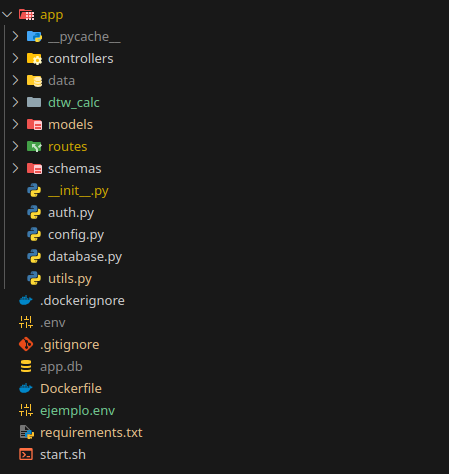
\includegraphics[width=0.7\linewidth]{img/EstructuraDeDirectorios/EstructuraBackend}
	\caption{Estructura de directorios del \textit{backend}.}
	\label{fig:estructurabackend}
\end{figure}


En cuanto al \textit{frontend} esta sería la estructura que se puede observar en la figura \ref{fig:estructurafrontend}.
\begin{figure}
	\centering
	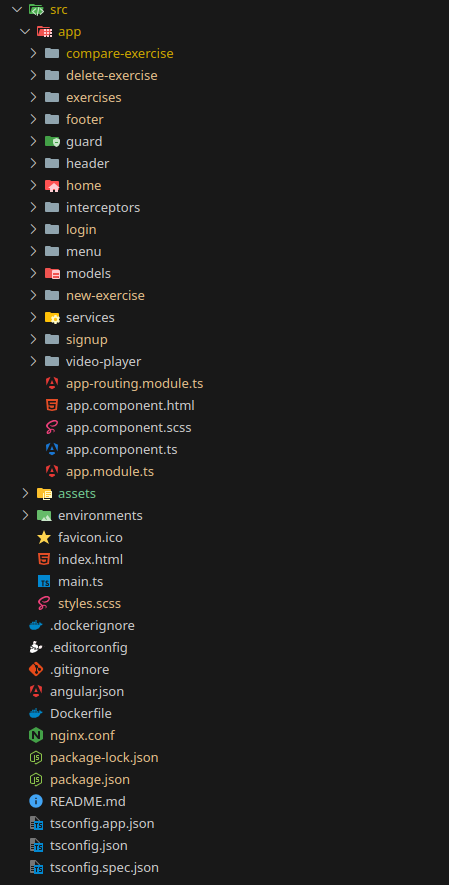
\includegraphics[width=0.7\linewidth]{img/EstructuraDeDirectorios/EstructuraFrontend}
	\caption{Estructura de directorios del \textit{frontend}.}
	\label{fig:estructurafrontend}
\end{figure}



\section{Manual del programador}

\begin{itemize}
	\item \textbf{Sistema operativo}: Para este proyecto se ha utilizado Arch Linux para desarrollar tanto la investigación como el desarrollo de la aplicación.
	\item \textbf{Versión de Python}: Durante el desarrollo se ha utilizado la versión 3.12 de Python.
\end{itemize}

\subsection{Notebooks}
Para ejecutar los \textit{notebooks} de Jupyter, se ha utilizado Visual Studio Code. Una vez se habrá por primera vez un \textit{notebook} en dicho programa, Visual Studio Code preguntará si se desea instalar las extensiones relacionadas con el tipo de archivo, es necesario responder de forma afirmativa.

\subsection{Aplicación Web}
La aplicación web se divide en varias partes, por lo que se tratará a continuación la instalación de cada parte por separado.
\begin{itemize}
	\item \textbf{Base de Datos}: Para ejecutar el proyecto es necesario tener instalado SQLite, que es la base de datos que se ha utilizado para el entorno de desarrollo ya que no requiere configuración para poderla usar.
	
	\item \textbf{API}: Para poder ejecutar la API es necesario tener instalada una versión de Python reciente. Concretamente se ha usado la 3.12. 
	
	\item \textbf{Frontend}: Para la aplicación web es necesario tener Angular 18 instalado y Node 22.4.
\end{itemize}

\section{Compilación, instalación y ejecución del proyecto}

\subsection{Descargar el repositorio}
Clonar el repositorio de GitHub mediante \textit{git clone} o descargar y descomprimir el ZIP que se puede obtener pulsando el botón \textit{Code} que se encuentra en la página de GitHub \cite{repo}.

\subsection{Entorno de Python}
Tanto para ejecutar los notebooks de Jupyter como la API es necesario crear y activar un entorno virtual de Python, para ello hay que ejecutar los comandos \ref{com:pythonvenv}. Una vez que se ha activado el entorno virtual es necesario instalarlas las dependencias mediante el comando \ref{com:pip}.

\begin{figure}
	\begin{lstlisting}[language=Bash]
		python -m venv .venv
		source .venv/bin/activate
	\end{lstlisting}
	\caption{Comandos para crear y activar entorno virtual de Python.}
	\label{com:pythonvenv}
\end{figure}

\begin{figure}
	\begin{lstlisting}[language=Bash]
		pip install -r requirements.txt
	\end{lstlisting}
	\caption{Comando para activar el entorno virtual de Python.}
	\label{com:pip}
\end{figure}

\subsection{API}
Para ejecutar la API es necesario ir al directorio \textit{app/backend} y renombrar el archivo \textit{ejemplo.env} de dicha carpeta a \textit{.env}. Después se puede o ejecutar el script \textit{start.sh} o ejecutar el comando  \ref{com:fastapidev} en el directorio \textit{app/backend}.

\begin{figure}
	\begin{lstlisting}[language=Bash]
		fastapi dev app
	\end{lstlisting}
	\caption{Comando para ejecutar el \textit{backend} en modo desarrollo.}
	\label{com:fastapidev}
\end{figure}
\subsection{Frontend}
En el caso del \textit{frontend}, al estar desarrollado en Angular, se puede compilar, para ello se puede ejecutar el comando \ref{com:ngbuild}.

A la hora de programar en modo desarrollo, resulta más sencillo ejecutar el comando \ref{com:ngserve} que recompila el código cada vez que detecta cambios en un archivo y lo ejecuta.
\begin{figure}
	\begin{lstlisting}[language=Bash]
		ng serve
	\end{lstlisting}
	\caption{Comando para ejecutar el \textit{frontend} en modo desarrollo.}
	\label{com:ngserve}
\end{figure}

\begin{figure}
	\begin{lstlisting}[language=Bash]
		ng build --prod
	\end{lstlisting}
	\caption{Comando para compilar el \textit{frontend} en modo producción.}
	\label{com:ngbuild}
\end{figure}
\subsection{Docker}
Para crear la red de contenedores de Docker basta con utilizar el siguiente comando \ref{com:dockercomposeup}. Esta red consta de tres contenedores, uno para la base de datos, otro para el \textit{backend} y otro para el \textit{frontend}.
\begin{figure}
	\begin{lstlisting}[language=Bash]
		docker compose up
	\end{lstlisting}
	\caption{Comando ejecutar los contenedores de docker.}
	\label{com:dockercomposeup}
\end{figure}
Añadir la opción \textit{--build} hace que los contenedores se recompilen, lo que será necesario si se hacen modificaciones en el código.
\section{Pruebas del sistema}
Las pruebas son fundamentales en el desarrollo de software porque permiten comprobar y validar que un sistema funciona correctamente. A través de las pruebas, se pueden identificar errores, fallos y problemas de rendimiento. Además, contribuyen a garantizar la calidad y fiabilidad del software, mejorando la experiencia del usuario y minimizando la necesidad de corregir errores en etapas avanzadas del desarrollo.

En este proyecto, se han llevado a cabo pruebas manuales para validar el software. Aunque las pruebas manuales pueden ser más laboriosas y consumir más tiempo, proporcionan flexibilidad y permiten una evaluación más detallada del software en términos de usabilidad, compatibilidad y funcionalidad. Esto es especialmente útil para interfaces de usuario complejas o interacciones específicas con el software que son difíciles de automatizar, como en el caso de esta aplicación.
